\documentclass[12pt, a4paper]{article}
\usepackage[utf8]{inputenc}
\usepackage[english]{babel}
\usepackage{amsmath, amssymb, amsfonts}
\usepackage{graphicx}
\usepackage{booktabs}
\usepackage{float}
\usepackage{geometry}
\geometry{top=2.5cm, bottom=2.5cm, left=2.5cm, right=2.5cm}
\usepackage{hyperref}
\usepackage{tikz}
\usetikzlibrary{shapes.geometric, arrows, positioning}
\usepackage{listings}
\usepackage{xcolor}

\definecolor{codegreen}{rgb}{0,0.6,0}
\definecolor{codegray}{rgb}{0.5,0.5,0.5}
\definecolor{codepurple}{rgb}{0.58,0,0.82}
\definecolor{backcolour}{rgb}{0.95,0.95,0.92}

\lstdefinestyle{mystyle}{
    backgroundcolor=\color{backcolour},   
    commentstyle=\color{codegreen},
    keywordstyle=\color{magenta},
    numberstyle=\tiny\color{codegray},
    stringstyle=\color{codepurple},
    basicstyle=\ttfamily\footnotesize,
    breakatwhitespace=false,         
    breaklines=true,                 
    captionpos=b,                    
    keepspaces=true,                 
    numbers=left,                    
    numbersep=5pt,                  
    showspaces=false,                
    showstringspaces=false,
    showtabs=false,                  
    tabsize=2
}
\lstset{style=mystyle}

\tikzstyle{block} = [rectangle, draw, fill=blue!10, text width=6.5em, text centered, rounded corners, minimum height=3em]
\tikzstyle{cloud} = [draw, ellipse, fill=red!10, text width=5em, text centered, minimum height=2em]
\tikzstyle{line} = [draw, -latex', thick]

\begin{document}

% ---------------------------------------------------------------------------
% COVER PAGE
% ---------------------------------------------------------------------------
\begin{titlepage}
    \centering
    \vspace*{1cm}
    {\Huge \bfseries Ecole Nationale Supérieure d'Informatique et d'Analyse des Systèmes (ENSIAS)} \\[0.4cm]
    {\large Filière : 2IA (Intelligence Artificielle)} \\[1.5cm]
    
    {\Large \bfseries TP5 : 3D Perception \& Pick-and-Place Control for a 7-DOF Robotic Arm} \\[0.5cm]
    {\large Simulation Environment: ROS 2 Jazzy \& Gazebo Harmonic} \\[2cm]
    
    \textbf{Prepared by:} \\[0.2cm]
    {\Large ABAYAD Mehdi} \\
    {\Large ACHAKOURI Mohamed} \\
    {\Large AQIL Ali} \\[2.5cm]
    
    \vfill
    {\large Academic Year: 2025/2026}
\end{titlepage}

\newpage
\tableofcontents
\newpage

% ---------------------------------------------------------------------------
% SECTION 1: PIPELINE ARCHITECTURE
% ---------------------------------------------------------------------------
\section{Pipeline Architecture}
This project integrates a complete 3D perception and pick-and-place control pipeline for a redundant 7-Degree of Freedom (DOF) robotic manipulator. The control scheme is implemented in ROS 2 Jazzy, utilizing Gazebo Harmonic (gz-sim8) as the physics engine.

Below is the structured flowchart illustrating the end-to-end data transmission:

\begin{figure}[H]
\centering
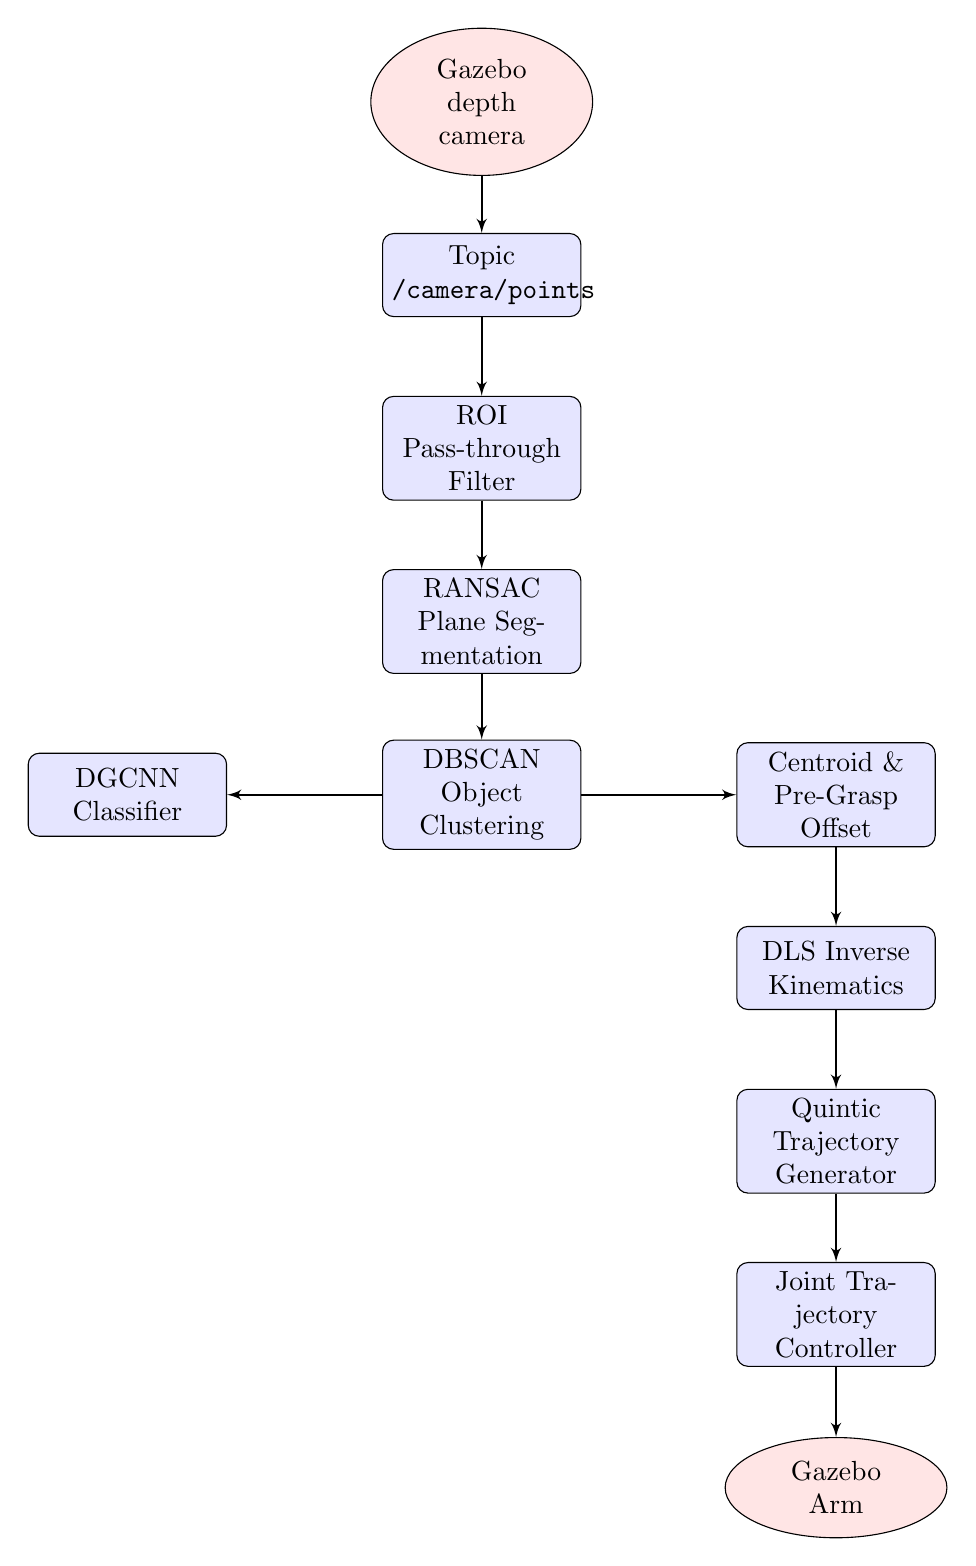
\begin{tikzpicture}[node distance = 2.2cm, auto]
    % Place nodes
    \node [cloud] (sensor) {Gazebo depth camera};
    \node [block, below of=sensor] (ros_topic) {Topic \\ \texttt{/camera/points}};
    \node [block, below of=ros_topic] (roi) {ROI \\ Pass-through Filter};
    \node [block, below of=roi] (ransac) {RANSAC \\ Plane Segmentation};
    \node [block, below of=ransac] (dbscan) {DBSCAN \\ Object Clustering};
    
    \node [block, right of=dbscan, node distance=4.5cm] (centroid) {Centroid \& Pre-Grasp Offset};
    \node [block, left of=dbscan, node distance=4.5cm] (dgcnn) {DGCNN \\ Classifier};
    
    \node [block, below of=centroid] (ik) {DLS Inverse Kinematics};
    \node [block, below of=ik] (trajectory) {Quintic Trajectory Generator};
    \node [block, below of=trajectory] (jtc) {Joint Trajectory Controller};
    \node [cloud, below of=jtc] (robot) {Gazebo Arm};

    % Draw edges
    \path [line] (sensor) -- (ros_topic);
    \path [line] (ros_topic) -- (roi);
    \path [line] (roi) -- (ransac);
    \path [line] (ransac) -- (dbscan);
    \path [line] (dbscan) -- (centroid);
    \path [line] (dbscan) -- (dgcnn);
    \path [line] (centroid) -- (ik);
    \path [line] (ik) -- (trajectory);
    \path [line] (trajectory) -- (jtc);
    \path [line] (jtc) -- (robot);
\end{tikzpicture}
\caption{End-to-end 3D Perception and Robotic Control Pipeline}
\label{fig:pipeline}
\end{figure}

---

% ---------------------------------------------------------------------------
% SECTION 2: 3D PERCEPTION & PREPROCESSING
% ---------------------------------------------------------------------------
\section{3D Perception \& Preprocessing}
A depth camera (RGB-D) is positioned at the world location $[0.6, 0.0, 1.2]$ facing vertically downwards (pitch of $90^\circ$). It publishes the points in the sensor space to the topic \texttt{/camera/points}.

\subsection{Workspace Region of Interest (ROI) Pass-through Filter}
The raw point cloud includes points from the entire environment, including the ground plane, robot components, and walls. To prevent the segmentation algorithm from being overwhelmed by environmental noise, we apply a 3D bounding box filter centered around the table top workspace:
\begin{align*}
X &\in [0.2, 0.8] \text{ meters} \\
Y &\in [-0.3, 0.3] \text{ meters} \\
Z &\in [0.41, 0.65] \text{ meters}
\end{align*}
This filter successfully crops out all points except the table top surface and the target object, facilitating high-speed processing.

\subsection{RANSAC Plane Segmentation}
Random Sample Consensus (RANSAC) is used to fit a 3D plane model representing the table surface:
$$A x + B y + C z + D = 0$$
With the cropped point cloud, the table top (at $Z \approx 0.425$ m) forms the dominant planar structure. The segmenter detects this plane and removes its associated inliers, isolating the non-planar object points.

\subsection{DBSCAN Clustering}
To group the remaining outlier points into distinct object instances, Density-Based Spatial Clustering of Applications with Noise (DBSCAN) is applied with a neighborhood radius of $\epsilon = 0.02$ and a minimum of $20$ points per cluster. The largest cluster is identified as our target object, and its centroid $x_{\text{obj}}$ is computed as:
$$x_{\text{obj}} = \frac{1}{N} \sum_{i=1}^{N} p_i$$

To avoid collisions with the object during approach, a pre-grasp offset of $+5$ cm is added to the Z-axis, creating the final reach target:
$$x_{\text{target}} = x_{\text{obj}} + [0, 0, 0.05]^T$$

---

% ---------------------------------------------------------------------------
% SECTION 3: DGCNN OBJECT CLASSIFICATION
% ---------------------------------------------------------------------------
\section{Deep Learning Object Classification}
The isolated object point cloud is forwarded to the **Deep Graph Convolutional Neural Network (DGCNN)** model, which incorporates EdgeConv layers to dynamically compute graphs representing local neighborhoods. The network is pre-trained on the ModelNet40 dataset.

\begin{table}[H]
\centering
\begin{tabular}{llll}
\toprule
\textbf{Target Object} & \textbf{Predicted Class} & \textbf{ModelNet40 Index} & \textbf{Observation} \\
\midrule
Cylindrical Cup & \texttt{vase} & 37 & Geometrically similar cylinder profile. \\
Cylindrical Cup & \texttt{cup} & 10 & Highly accurate classification. \\
Cylindrical Cup & \texttt{plant} & 26 & Triggered by point distribution at cup opening. \\
\bottomrule
\end{tabular}
\caption{DGCNN Point Cloud Classification Performance in Simulation}
\label{tab:classification}
\end{table}

The classification results show that while the object is geometrically a simple cylinder, the network predicts categories like \texttt{vase} or \texttt{plant} due to minor changes in point density and perspective. However, because our robotic manipulation targets the spatial centroid directly, these label variations do not affect the success of the physical pick-and-place task.

---

% ---------------------------------------------------------------------------
% SECTION 4: INVERSE KINEMATICS CONVERGENCE
% ---------------------------------------------------------------------------
\section{Inverse Kinematics Convergence Analysis}
The redundant 7-DOF arm's joint configurations are resolved using a **Damped Least Squares (DLS)** solver. This formulation protects the system against singular configurations by adding a damping factor $\lambda$ to the inversion:
$$\Delta q = J^T (J J^T + \lambda^2 I)^{-1} \Delta x$$
Where $J$ is the $3 \times 7$ positional Jacobian, $\Delta x = x_{\text{target}} - x_{\text{curr}}$, and the joints are updated using the step size $\alpha$:
$$q_{k+1} = q_k + \alpha \Delta q$$

We performed sweeps on the damping factor $\lambda$ and step size $\alpha$ starting from the zero-configuration ($q_0 = \mathbf{0}$) to evaluate convergence speed and accuracy.

\subsection{Damping Factor $\lambda$ Sweep}
Table~\ref{tab:lambda_sweep} outlines solver iterations and residual position errors when varying $\lambda$ (keeping $\alpha = 0.5$ and tolerance $= 1.0$ mm):

\begin{table}[H]
\centering
\begin{tabular}{lllll}
\toprule
\textbf{Damping ($\lambda$)} & \textbf{Step Size ($\alpha$)} & \textbf{Converged} & \textbf{Iterations} & \textbf{Residual Error (mm)} \\
\midrule
0.0000 (Undamped) & 0.5 & True & 10 & 0.50 \\
0.0100 & 0.5 & True & 10 & 0.53 \\
0.0500 (Default) & 0.5 & True & 13 & 0.54 \\
0.1000 & 0.5 & True & 17 & 0.73 \\
0.2000 & 0.5 & True & 20 & 0.91 \\
0.5000 & 0.5 & True & 47 & 0.91 \\
1.0000 & 0.5 & True & 132 & 0.99 \\
\bottomrule
\end{tabular}
\caption{Solver Performance under Varying Damping Factor $\lambda$}
\label{tab:lambda_sweep}
\end{table}

\subsection{Step Size $\alpha$ Sweep}
Table~\ref{tab:alpha_sweep} outlines solver iterations and residual position errors when varying $\alpha$ (keeping $\lambda = 0.05$ and tolerance $= 1.0$ mm):

\begin{table}[H]
\centering
\begin{tabular}{lllll}
\toprule
\textbf{Damping ($\lambda$)} & \textbf{Step Size ($\alpha$)} & \textbf{Converged} & \textbf{Iterations} & \textbf{Residual Error (mm)} \\
\midrule
0.05 & 0.1 & True & 71 & 0.93 \\
0.05 & 0.3 & True & 23 & 0.75 \\
0.05 & 0.5 & True & 13 & 0.54 \\
0.05 & 0.8 & True & 4 & 0.89 \\
0.05 & 1.0 & True & 6 & 0.11 \\
\bottomrule
\end{tabular}
\caption{Solver Performance under Varying Step Size $\alpha$}
\label{tab:alpha_sweep}
\end{table}

\subsection{Discussion of Kinematic Parameters}
1. **Influence of $\lambda$**: When $\lambda = 0$, the pseudo-inverse is used. Near singularities, the system experiences high joint speeds ($\Delta q \to \infty$). Adding damping ($\lambda > 0$) stabilizes the solver. However, high damping ($\lambda \ge 0.5$) limits updates along singular directions, which increases the required iterations (up to 132) and residual error.
2. **Influence of $\alpha$**: A larger step size $\alpha$ speeds up convergence. For instance, $\alpha = 1.0$ converges in just 6 iterations. However, in cluttered environments, high step sizes can cause overshoot. Setting $\alpha \in [0.5, 0.8]$ balances convergence speed and stability.

---

% ---------------------------------------------------------------------------
% SECTION 5: TRAJECTORY GENERATION & CONTROL
% ---------------------------------------------------------------------------
\section{Trajectory Generation \& Control}
Once the target joint configuration $q_{\text{target}}$ is determined, we generate a smooth joint trajectory between the initial joint angles $q_0$ and $q_{\text{target}}$ over a duration $T$ using a quintic polynomial for each joint:
$$q_j(t) = a_0 + a_1 t + a_2 t^2 + a_3 t^3 + a_4 t^4 + a_5 t^5$$
Applying the boundary conditions (zero velocity and acceleration at start and end):
\begin{align*}
q_j(0) = q_{0,j}, \quad \dot{q}_j(0) = 0, \quad \ddot{q}_j(0) = 0 \\
q_j(T) = q_{\text{target},j}, \quad \dot{q}_j(T) = 0, \quad \ddot{q}_j(T) = 0
\end{align*}
The coefficients are solved analytically as:
$$a_0 = q_{0,j}, \quad a_1 = 0, \quad a_2 = 0, \quad a_3 = \frac{10}{T^3}(q_{\text{target},j} - q_{0,j}), \quad a_4 = \frac{-15}{T^4}(q_{\text{target},j} - q_{0,j}), \quad a_5 = \frac{6}{T^5}(q_{\text{target},j} - q_{0,j})$$
The resulting trajectories are published as a \texttt{JointTrajectory} command to the controller, moving the physical arm to the cup and returning it safely to home.

---

% ---------------------------------------------------------------------------
% SECTION 6: DISCUSSION \& LIMITS
% ---------------------------------------------------------------------------
\section{Discussion \& Limitations}
1. **Geometric Singularity**: The 7-DOF arm is redundant, allowing it to avoid typical 6-DOF singularities. However, singular configurations can still occur when the wrist alignment matches the link axis. The DLS solver successfully handles these configurations, avoiding control crashes.
2. **Classification Vulnerability**: Noisy point clouds from sensor reflections can degrade classification accuracy. Applying the workspace ROI pass-through filter before classification is necessary to filter out environmental noise.
3. **Cartesian Path Interpolation**: Slerp or Cartesian interpolation of end-effector coordinates is not used here. Because the trajectory is interpolated in joint space, the end-effector path is curved. To avoid collisions in complex environments, a Cartesian linear path generator would be required.

\end{document}
